In the beginning and the end of the genetics accelerator pipeline lies the rated and the unrated pools, respectively.
The rated and unrated pools are caches of genetics individuals that waiting to either 1) get selected and be sent through the pipeline, 2) die, or 3) get picked up by a fitness core for fitness ranking.
The rated pool contains individuals stored with a fitness score, and are the indivuiduals that have just been inserted into the accelerator by a fitness core.
The unrated pool contains individuals that have no fitness score calculated.
They are the new individuals produced by the accelerator pipeline, and are waiting to be picked up and rated by a fitness core.

The rated and unrated pools are implemented in \gls{BRAM} on the FPGA for as fast access times as possible.
This is essential to achieve a high memory throughput when executing the algorithms.

It is important to note that the two pools are designed as separate \gls{BRAM} devices.
This is done to achieve even better memory throughput.
The increased throughput is achieved because the different computational units can work on the rated and unrated pools simultaneously.
For instance while one fitness core is storing a ranked individual, another fitness core may be fetching a new individual for ranking. 

Access to both the rated pool and the unrated pool is arbitraged by a controller referred to as the \gls{genetic controller}.
As with the \gls{data controller} for data memory access, the \gls{genetic controller} is responsible for granting access to the rated and unrated pool.
As shown in figure x\cn\todo{ref the architecture figure}, the genetics accelerator has its own data buses connected to the fitness cores separate from the data bus that is connected to the regular shared data memory.

The \gls{genetic controller} is based on the same principle as the \gls{data controller} described in section \vref{subsec:fpga-data-memory}.
When performing genetic operations, the fitness cores need to request the data bus by using two request signals.
The combination of these signals refer to the operation the fitness core requests from the genetic controller. 

The genetic controller continuously performs a simple round-robin request handling scheme in order to grant bus access to the requesting fitness cores, and to the genetic pipeline.
The logic surrounding the different operations are implemented as an state machine to divide the operations in different clock cycles.
This is the same method as is used in the data controller.

The state machine is shown in figure \ref{fpga:fig:mem:genetic_memory_ctrl}.

\begin{figure}

  \centering
  % Trim er [left bottom right top]
  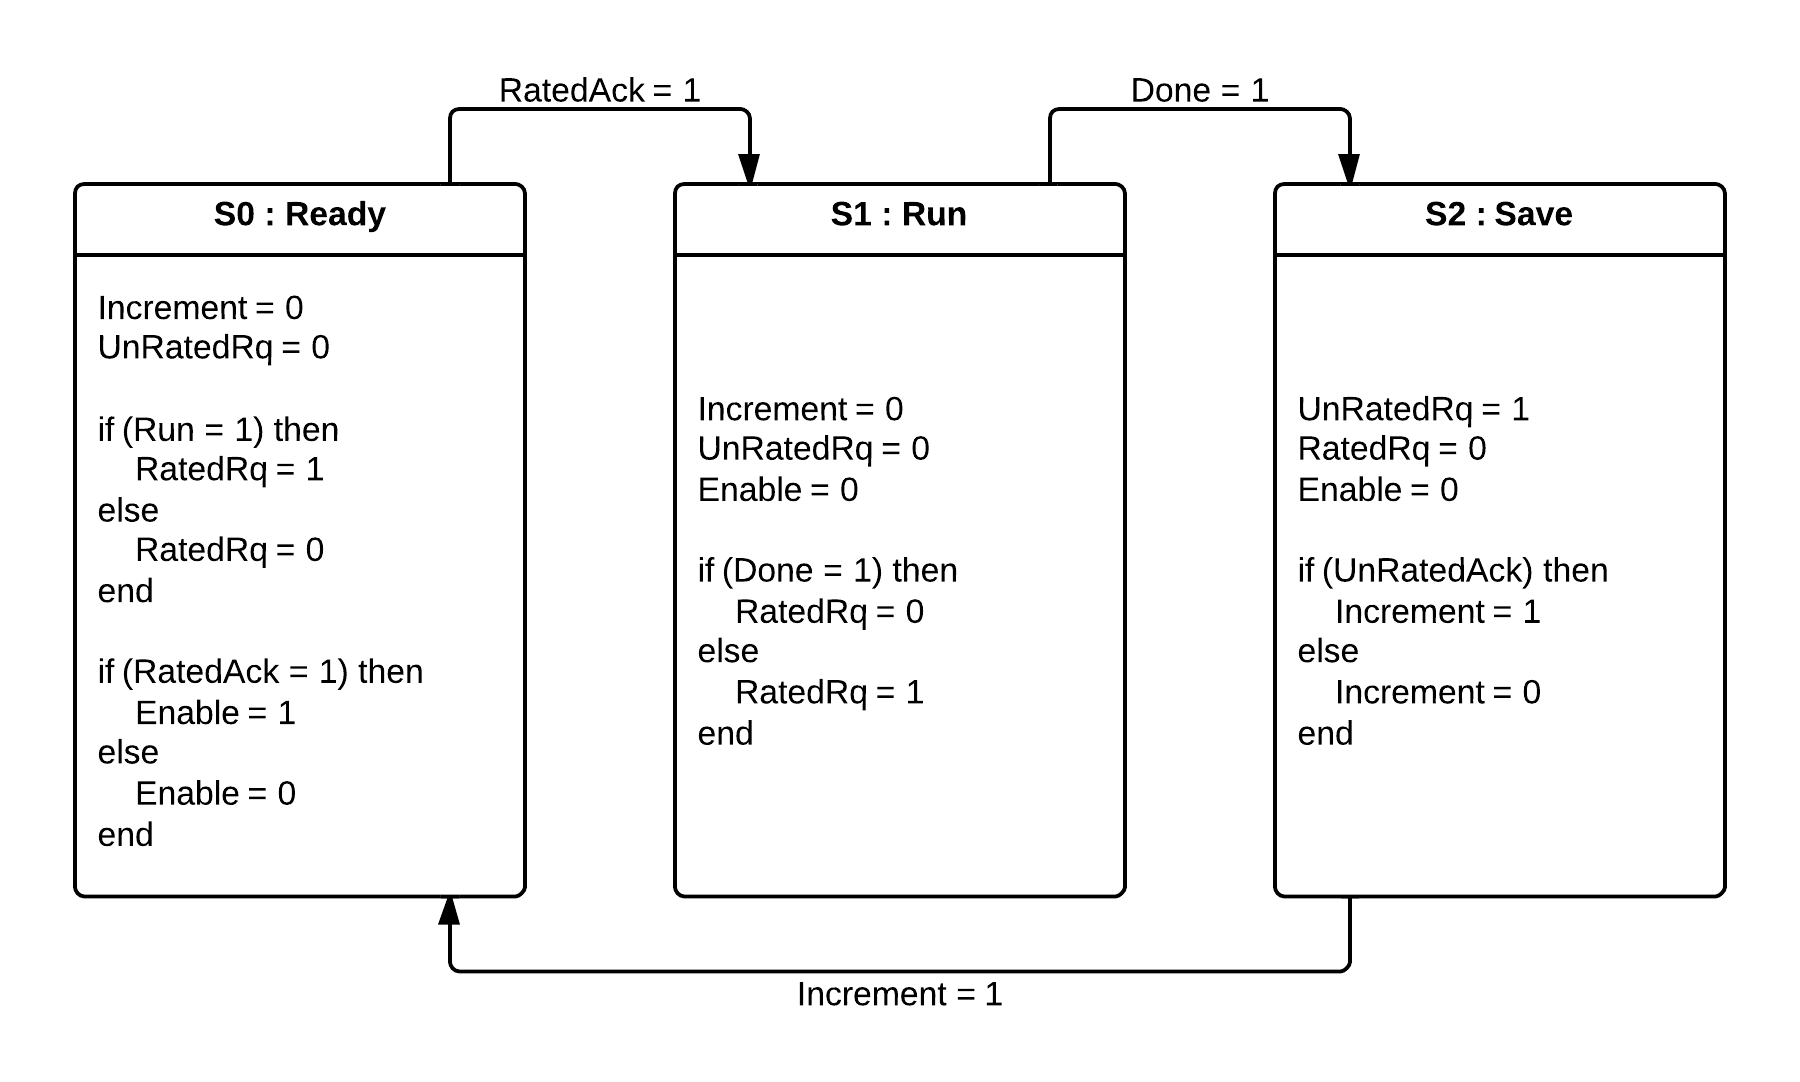
\includegraphics[width=\textwidth]{fpga/fig/genetic_ctrl.png}
  \caption{Genetic memory controller state machine}
  \label{fpga:fig:mem:genetic_memory_ctrl}
\end{figure}
